\newpage
\section{Diagrammi di sequenza}

\subsection{Front-End}
I seguenti diagrammi di sequenza prendono in considerazione le principali operazioni del front-end e vanno ad illustrarne le interazioni tra le classi.

\subsubsection{Registrazione utente}

\begin{figure}[H]
	\centering
	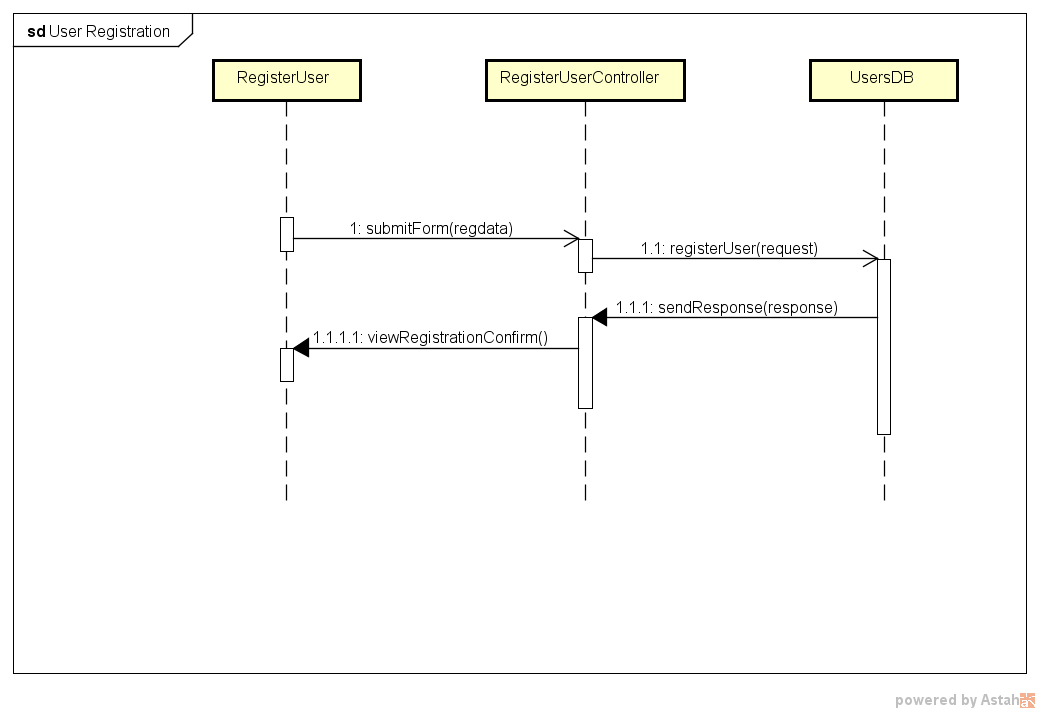
\includegraphics
	[width=0.7\linewidth]
	{UML/DiagrammiSequenza/registrazione_utente.png}
	\caption{Diagramma di sequenza: Registrazione utente}
\end{figure}

\begin{itemize}
	\item \textbf{Pre-condizioni}: l'utente si trova nella schermata di registrazione utente;
	\item \textbf{Post-condizioni}: l'utente ha compilato il form per la registrazione ed ora possiede le credenziali per l'autenticazione alla piattaforma API Market;
	\item \textbf{Descrizione}: l'utente compila il form per la registrazione di un account, provvedendo ad inserire tutte le informazioni obbligatorie richieste. Confermando la registrazione, i services di API Market provvedono ad inserire nel database il nuovo utente. A registrazione avvenuta, l'utente riceve un messaggio di successo e viene reindirizzato alla pagina di login.
\end{itemize}


\subsubsection{Autenticazione}

\begin{figure}[H]
	\centering
	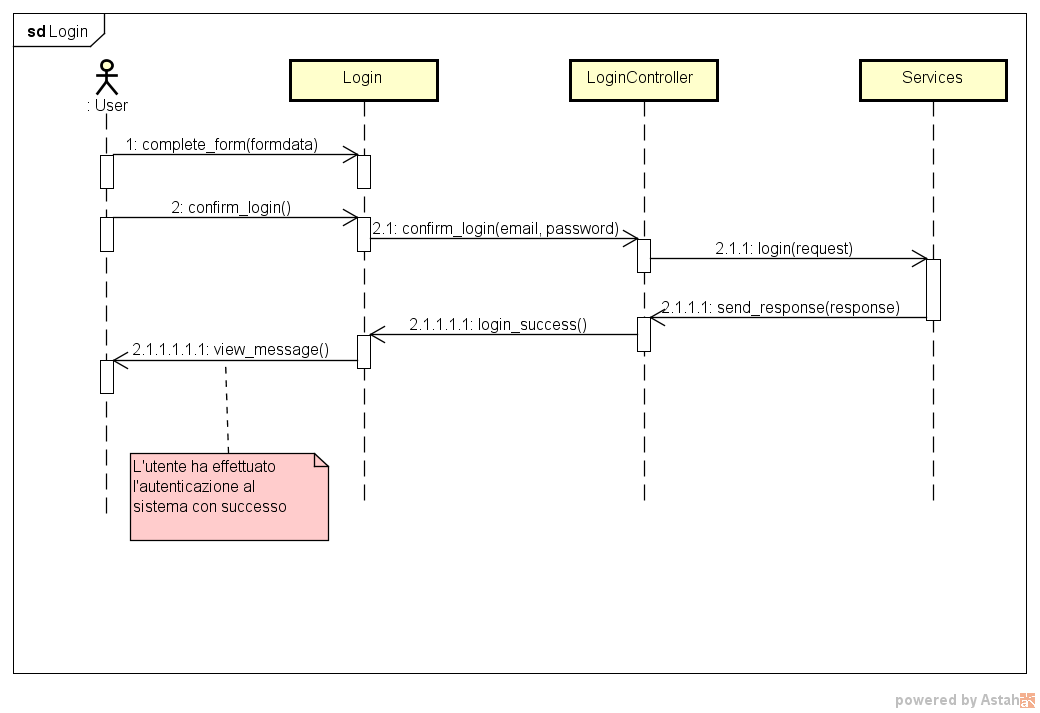
\includegraphics
	[width=0.7\linewidth]
	{UML/DiagrammiSequenza/login.png}
	\caption{Diagramma di sequenza: Autenticazione}
\end{figure}

\begin{itemize}
	\item \textbf{Pre-condizioni}: l'utente si trova nella schermata di autenticazione;
	\item \textbf{Post-condizioni}: l'utente ha compilato il form per il login ed ora risulta un utente autenticato al sistema API Market;
	\item \textbf{Descrizione}: l'utente compila il form per l'autenticazione, provvedendo ad inserire la propria email e password con le quali si era registrato. Confermando l'autenticazione, la piattaforma API Market provvede a creare una sessione per l'utente autenticato, il quale, nel caso di autenticazione avvenuta con successo, viene reindirizzato alla home dell'applicazione.
\end{itemize}
\clearpage

\subsubsection{Recupero password}

\begin{figure}[H]
	\centering
	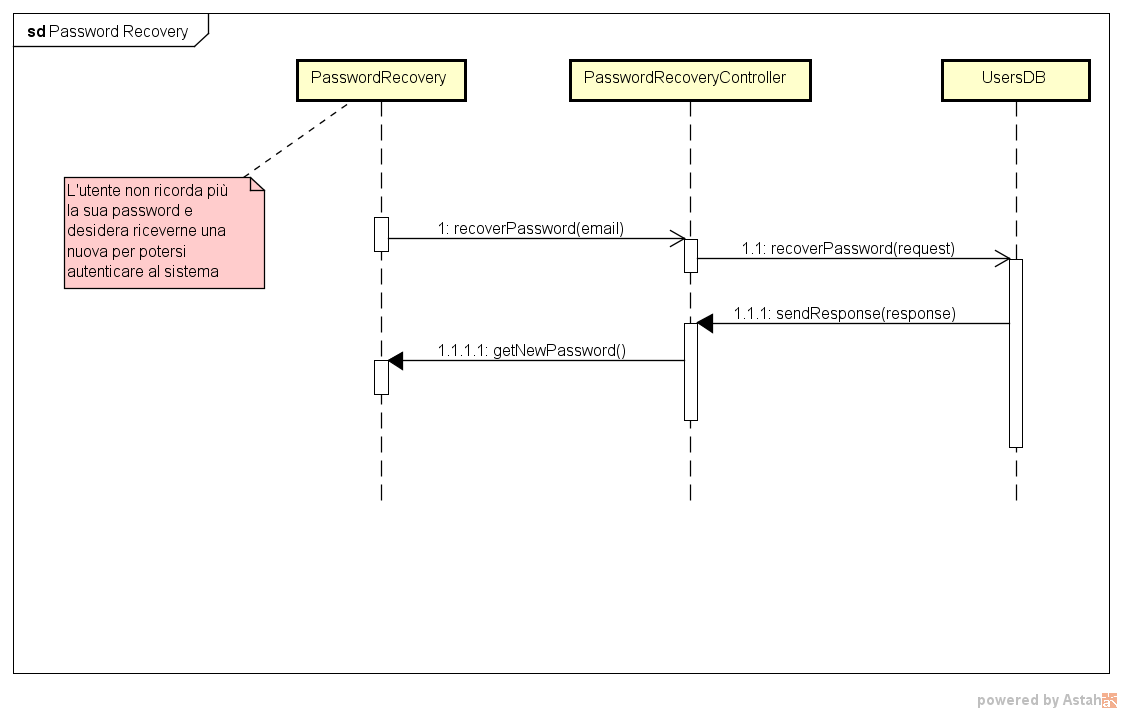
\includegraphics
	[width=0.7\linewidth]
	{UML/DiagrammiSequenza/recupero_password.png}
	\caption{Diagramma di sequenza: Recupero password}
\end{figure}

\begin{itemize}
	\item \textbf{Pre-condizioni}: l'utente si trova nella schermata di recupero password;
	\item \textbf{Post-condizioni}: l'utente ha compilato il form per il recupero della propria password tramite email ed ora può ri-effettuare l'autenticazione alla piattaforma API Market;
	\item \textbf{Descrizione}: l'utente compila il form per il recupero della password relativa al proprio account, inserendo l'email dove il sistema inoltrerà la nuova password generata. Confermando l'operazione, i services di API Market provvedono ad aggiornare il campo password nel database degli utenti. A recupero avvenuto, l'utente riceve un messaggio di successo e viene reindirizzato alla pagina di login.
\end{itemize}
\clearpage

\subsubsection{Ricerca API}

\begin{figure}[H]
	\centering
	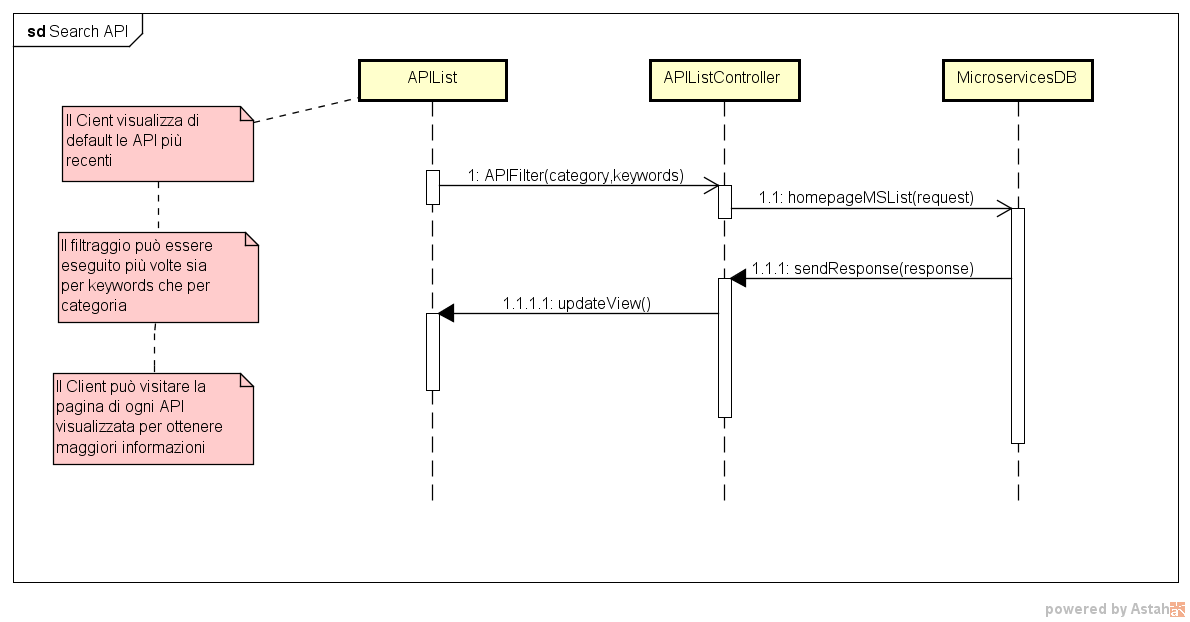
\includegraphics
	[width=0.7\linewidth]
	{UML/DiagrammiSequenza/ricercaAPI.png}
	\caption{Diagramma di sequenza: Ricerca API}
\end{figure}

\begin{itemize}
	\item \textbf{Pre-condizioni}: l'utente si trova nella homepage dell'applicazione;
	\item \textbf{Post-condizioni}: l'utente ha visualizzato le API secondo la categoria e le keywords inserite;
	\item \textbf{Descrizione}: di default, la homepage di API Market mostra le API registrate più recentemente. L'utente può immettere delle keywords nell'apposito riquadro per alterare i risultati, e scegliere di restringere la ricerca ad una singola categoria. I risultati visualizzati cambiano dinamicamente non appena l'applicazione web riceve risposta dai servizi che la collegano ai database.
\end{itemize}
\clearpage

\subsubsection{Acquisto API}

\begin{figure}[H]
	\centering
	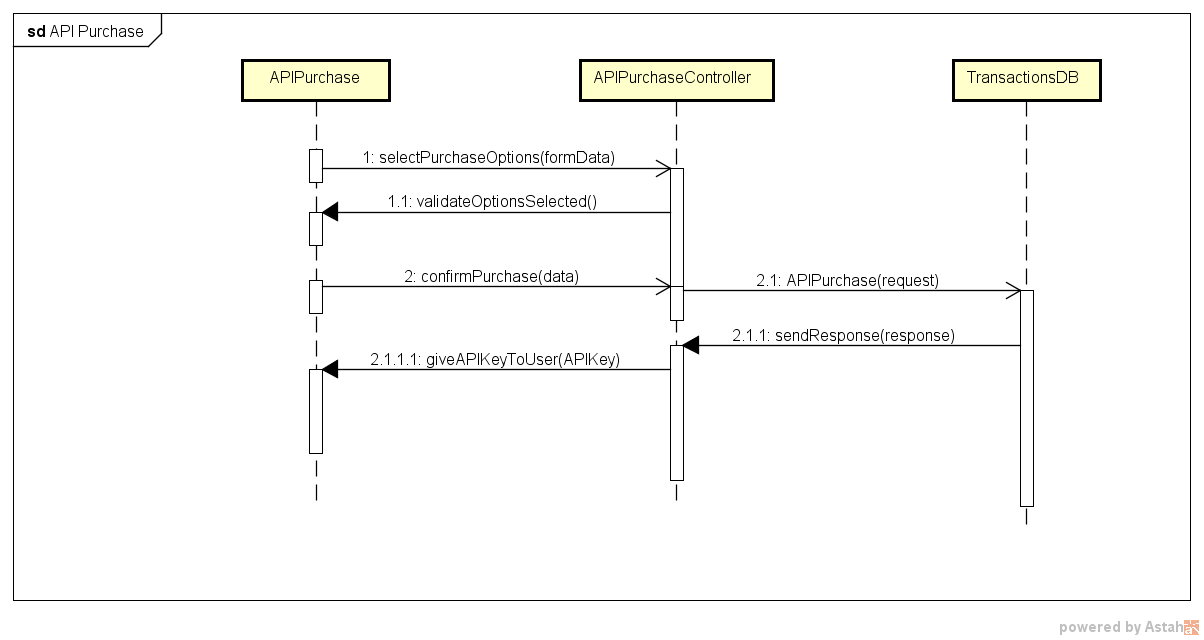
\includegraphics
	[width=0.7\linewidth]
	{UML/DiagrammiSequenza/acquistoAPI.png}
	\caption{Diagramma di sequenza: Acquisto API}
\end{figure}

\begin{itemize}
	\item \textbf{Pre-condizioni}: il cliente si trova nella schermata di acquisto di una specifica API;
	\item \textbf{Post-condizioni}: il cliente ha ricevuto l'API Key per l'API acquistata, secondo le modalità da lui scelte, e gli sono stati sottratti i corrispondenti crediti;
	\item \textbf{Descrizione}: il cliente compila il form per l'acquisto dell'API desiderata, visualizzando il preventivo di crediti spesi in base ai parametri scelti. Confermando l'acquisto (che può essere anche un rinnovo), i services di API Market provvedono a generare una apikey ed a scalare i crediti dall'account utente. L'utente potrà visualizzare l'API Key ed un messaggio di ringraziamento.
\end{itemize}

\subsubsection{Inserimento API}

\begin{figure}[H]
	\centering
	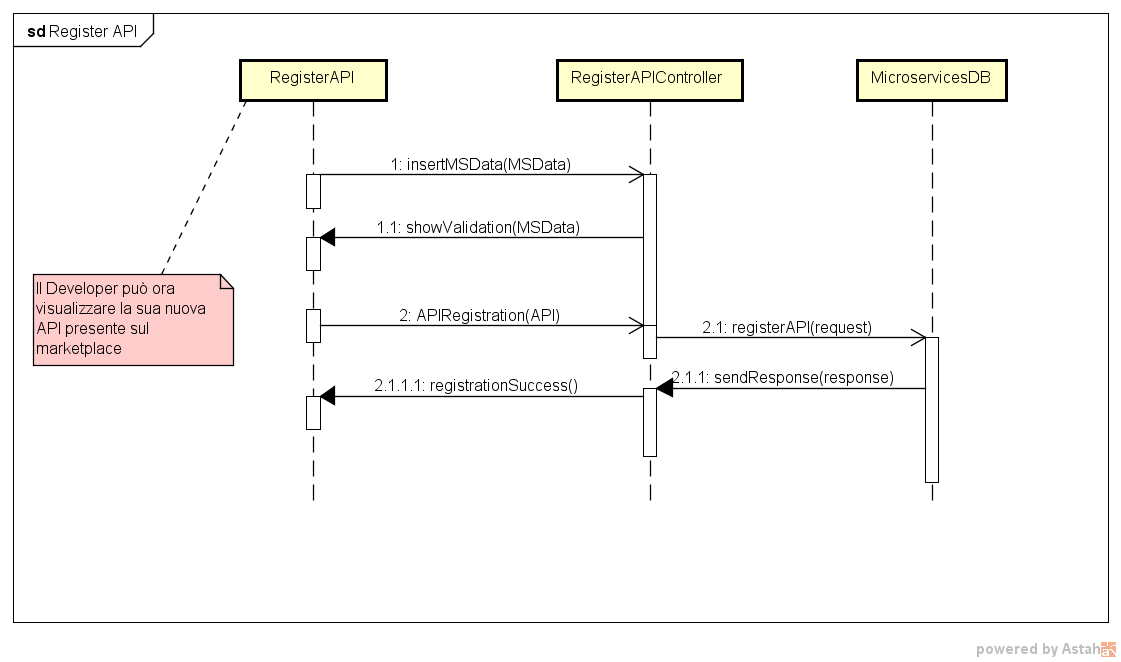
\includegraphics
	[width=0.7\linewidth]
	{UML/DiagrammiSequenza/registrazioneAPI.png}
	\caption{Diagramma di sequenza: Inserimento API}
\end{figure}

\begin{itemize}
	\item \textbf{Pre-condizioni}: lo sviluppatore si trova nella schermata di registrazione di una nuova API;
	\item \textbf{Post-condizioni}: lo sviluppatore ha registrato la sua nuova API ed essa è ora disponibile in API Market;
	\item \textbf{Descrizione}: lo sviluppatore compila il form per la registrazione di una nuova API, provvedendo anche a caricare sul server di API Market i file del logo e della documentazione PDF. Confermando la registrazione, i services di API Market provvedono ad inserire nel database la nuova API e renderla accessibile attraverso il Gateway. A registrazione avvenuta, lo sviluppatore riceve un messaggio di successo.
\end{itemize}
\clearpage

\subsubsection{Ricarica saldo conto virtuale}

\begin{figure}[H]
	\centering
	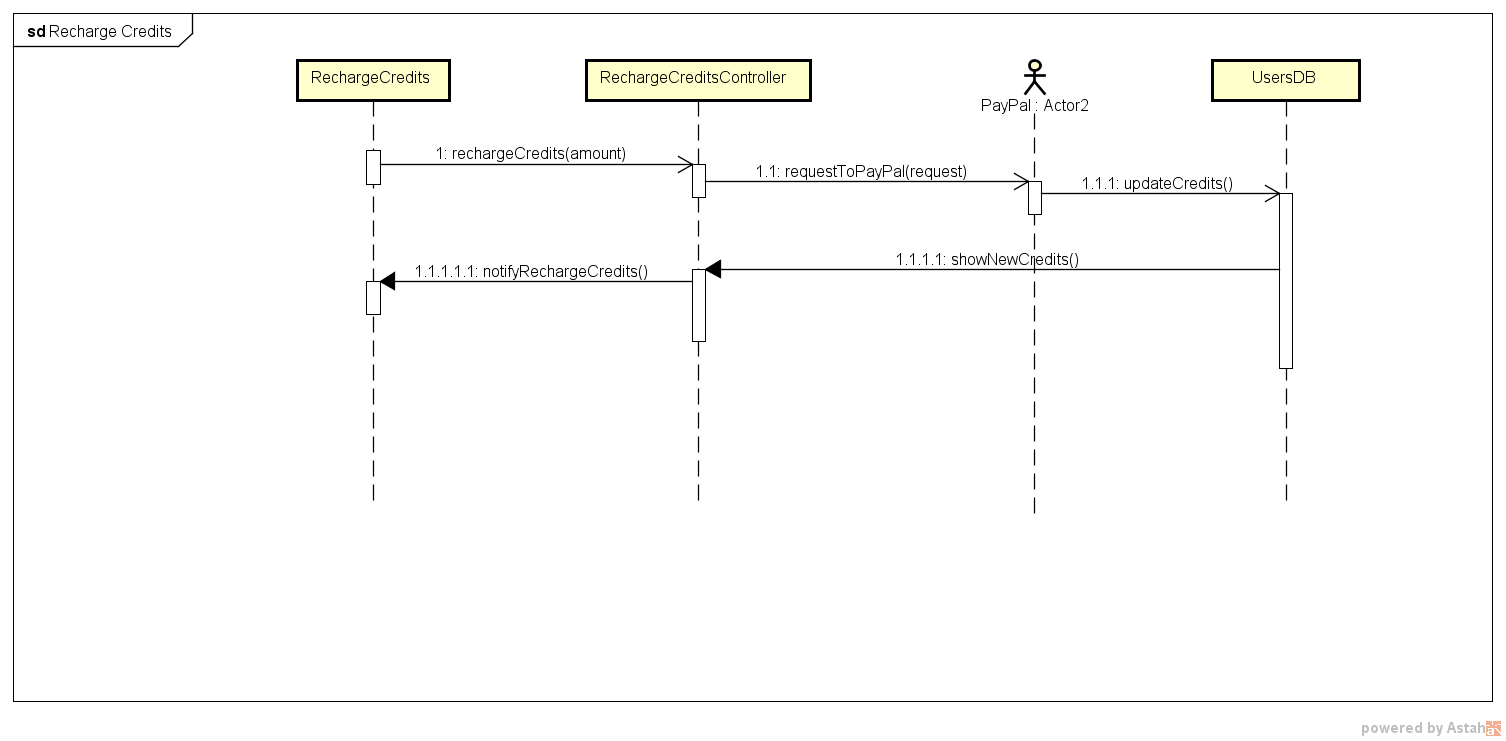
\includegraphics
	[width=0.7\linewidth]
	{UML/DiagrammiSequenza/ricaricaCrediti.png}
	\caption{Diagramma di sequenza: Ricarica saldo conto virtuale}
\end{figure}

\begin{itemize}
	\item \textbf{Pre-condizioni}: il cliente si trova nella schermata di ricarica del proprio conto virtuale;
	\item \textbf{Post-condizioni}: il cliente ha effettuato la ricarica dei propri crediti;
	\item \textbf{Descrizione}: il cliente stabilisce l'ammontare dei crediti da ricaricare nel proprio conto virtuale. A decisione avvenuta, verrà reindirizzato alla procedura di acquisto di PayPal, che lo guiderà nell'acquisto. Portata a termine la transazione, PayPal avvertirà i services di API Market che si occuperanno di incrementare i crediti del conto virtuale del cliente.
\end{itemize}


%\subsection{Back-End}
%I seguenti diagrammi di sequenza prendono in considerazione le principali operazioni del back-end e vanno ad illustrarne le interazioni tra le classi.
